\documentclass[12pt]{beamer}
\usetheme{Freiburg}
%\usepackage{german}
\usepackage{hyperref}
\usepackage{eurosym}



\mode<presentation>
\setbeamercolor{palette secondary}{fg=white,bg=white} 
\setbeamercolor{block title}{fg=white,bg=craneblue!80}
\setbeamercolor{block body}{parent=normal text,use=block title, bg=block title.bg!25!bg}


\mode
<all>
\beamertemplatenavigationsymbolsempty



\begin{document}

\title[]{\textbf{GIS+ Project}}   
\subtitle{Rasterizer}
\author[]{Luka Kern, Nele Stackelberg and Felix Rentschler}
\institute{University of Freiburg}
\date{July 5th, 2018}
%\logo{\includegraphics[scale=0.14]{logoKopie}}
%\setbeamercolor{logo}{fg=white,bg=white}

\begin{frame}
\titlepage
\end{frame}


\section{Task} 
\begin{frame}\frametitle{Task: Rasterizer}
\hspace{0.5cm}
\begin{figure}
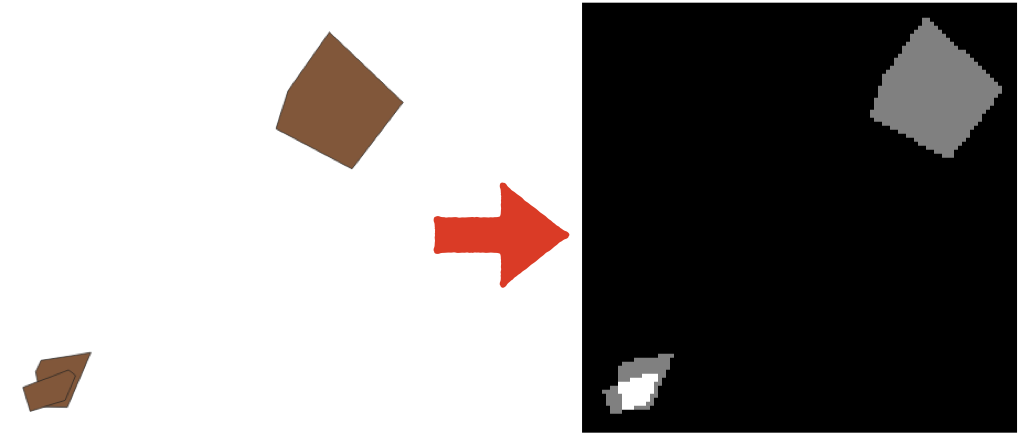
\includegraphics[scale=0.20]{rasterizer.png}\

\caption{from shape to raster}
\end{figure}
\end{frame}

\section{Structure of the Function}


\subsection{Load Shapefile}
\begin{frame}\frametitle{Load Shapefile with Fiona Package}

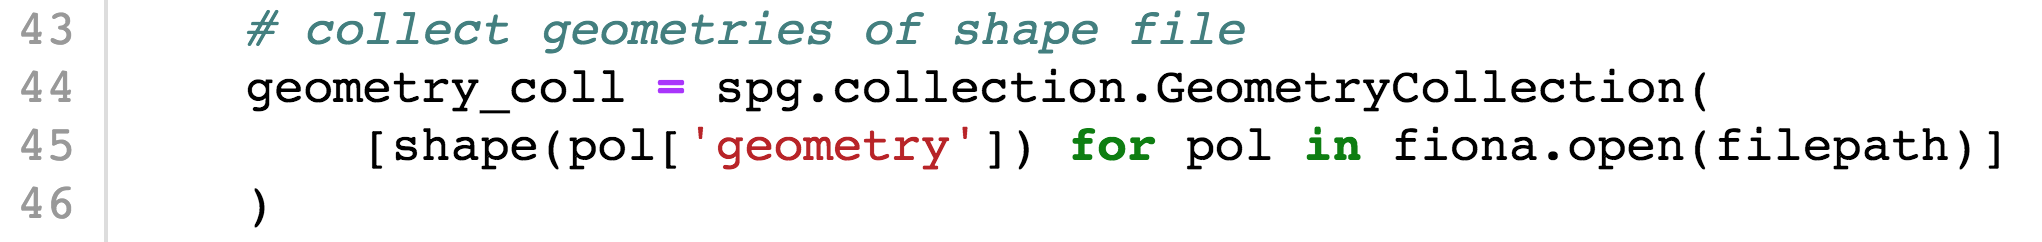
\includegraphics[scale=0.27]{fiona2.png}
\end{frame}


\subsection{Bounding Box}
\begin{frame}\frametitle{Bounding Box}
\hspace{0.5cm}
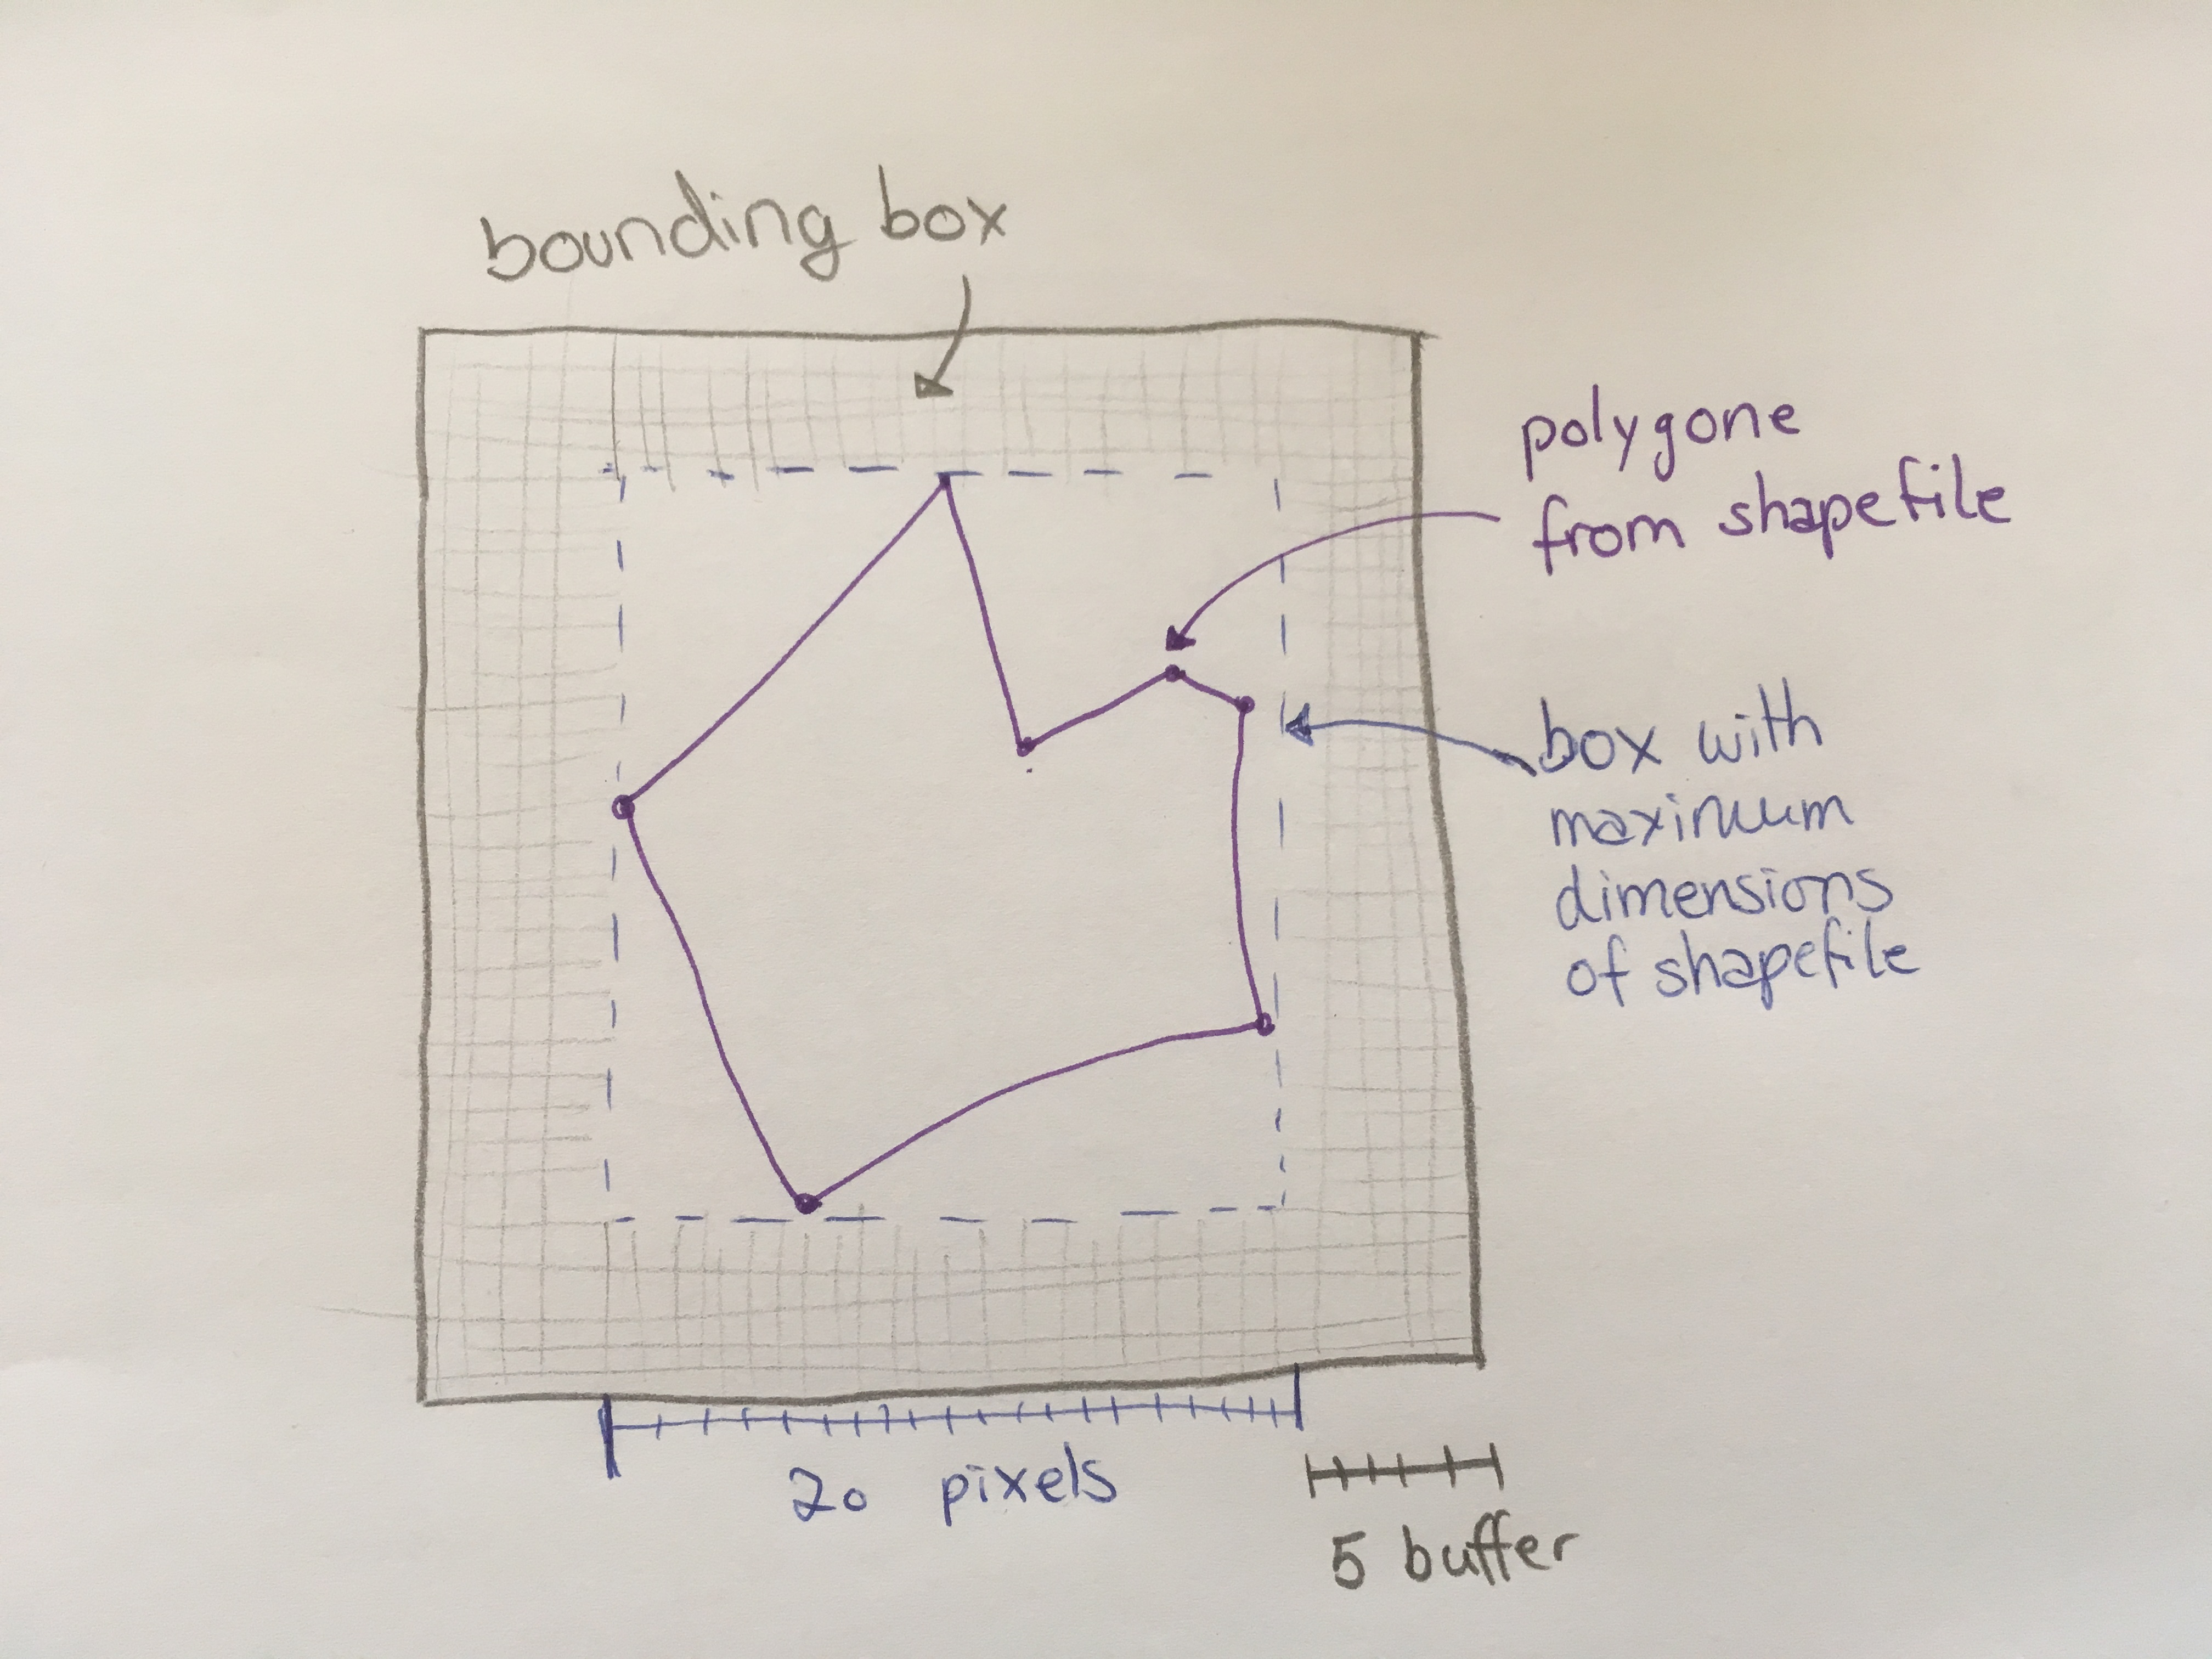
\includegraphics[scale=0.06]{IMG_5505.JPG}
\end{frame}


\subsection{Create Grid}
\begin{frame}\frametitle{Create a grid}
\hspace{0.5cm}
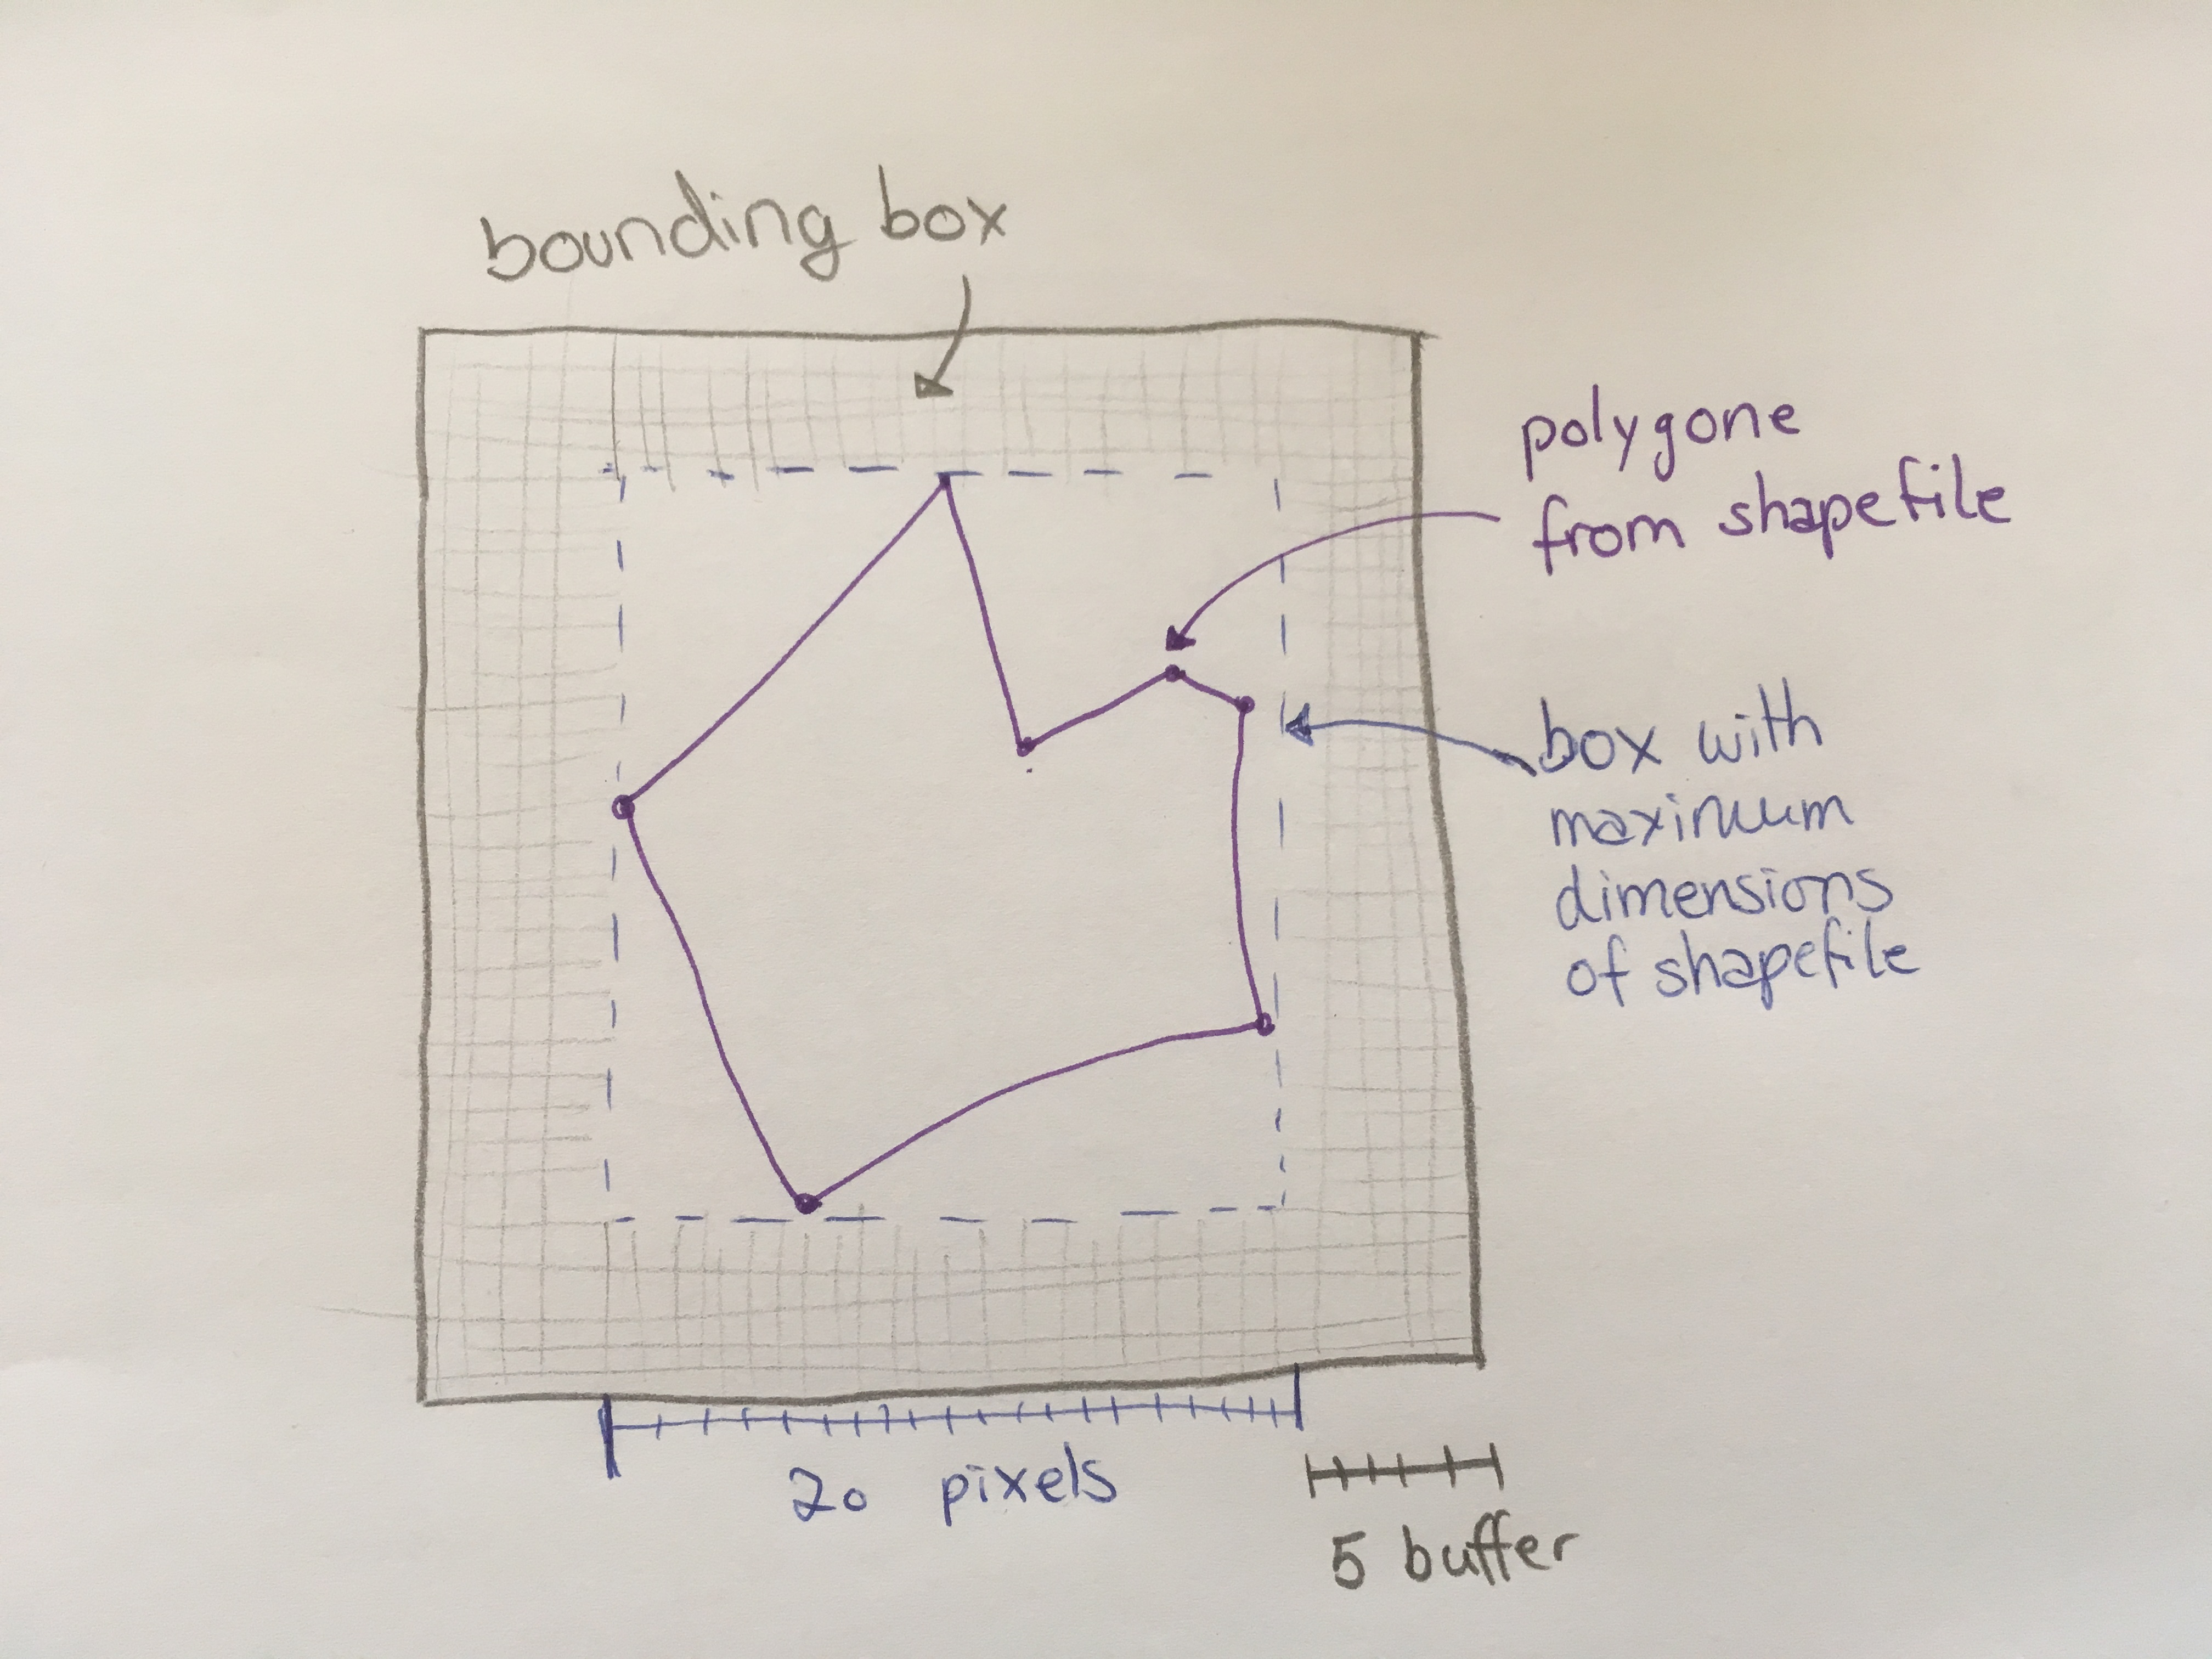
\includegraphics[scale=0.06]{IMG_5505.JPG}
\end{frame}


\subsection{Within Query}

\begin{frame}\frametitle{Within query}

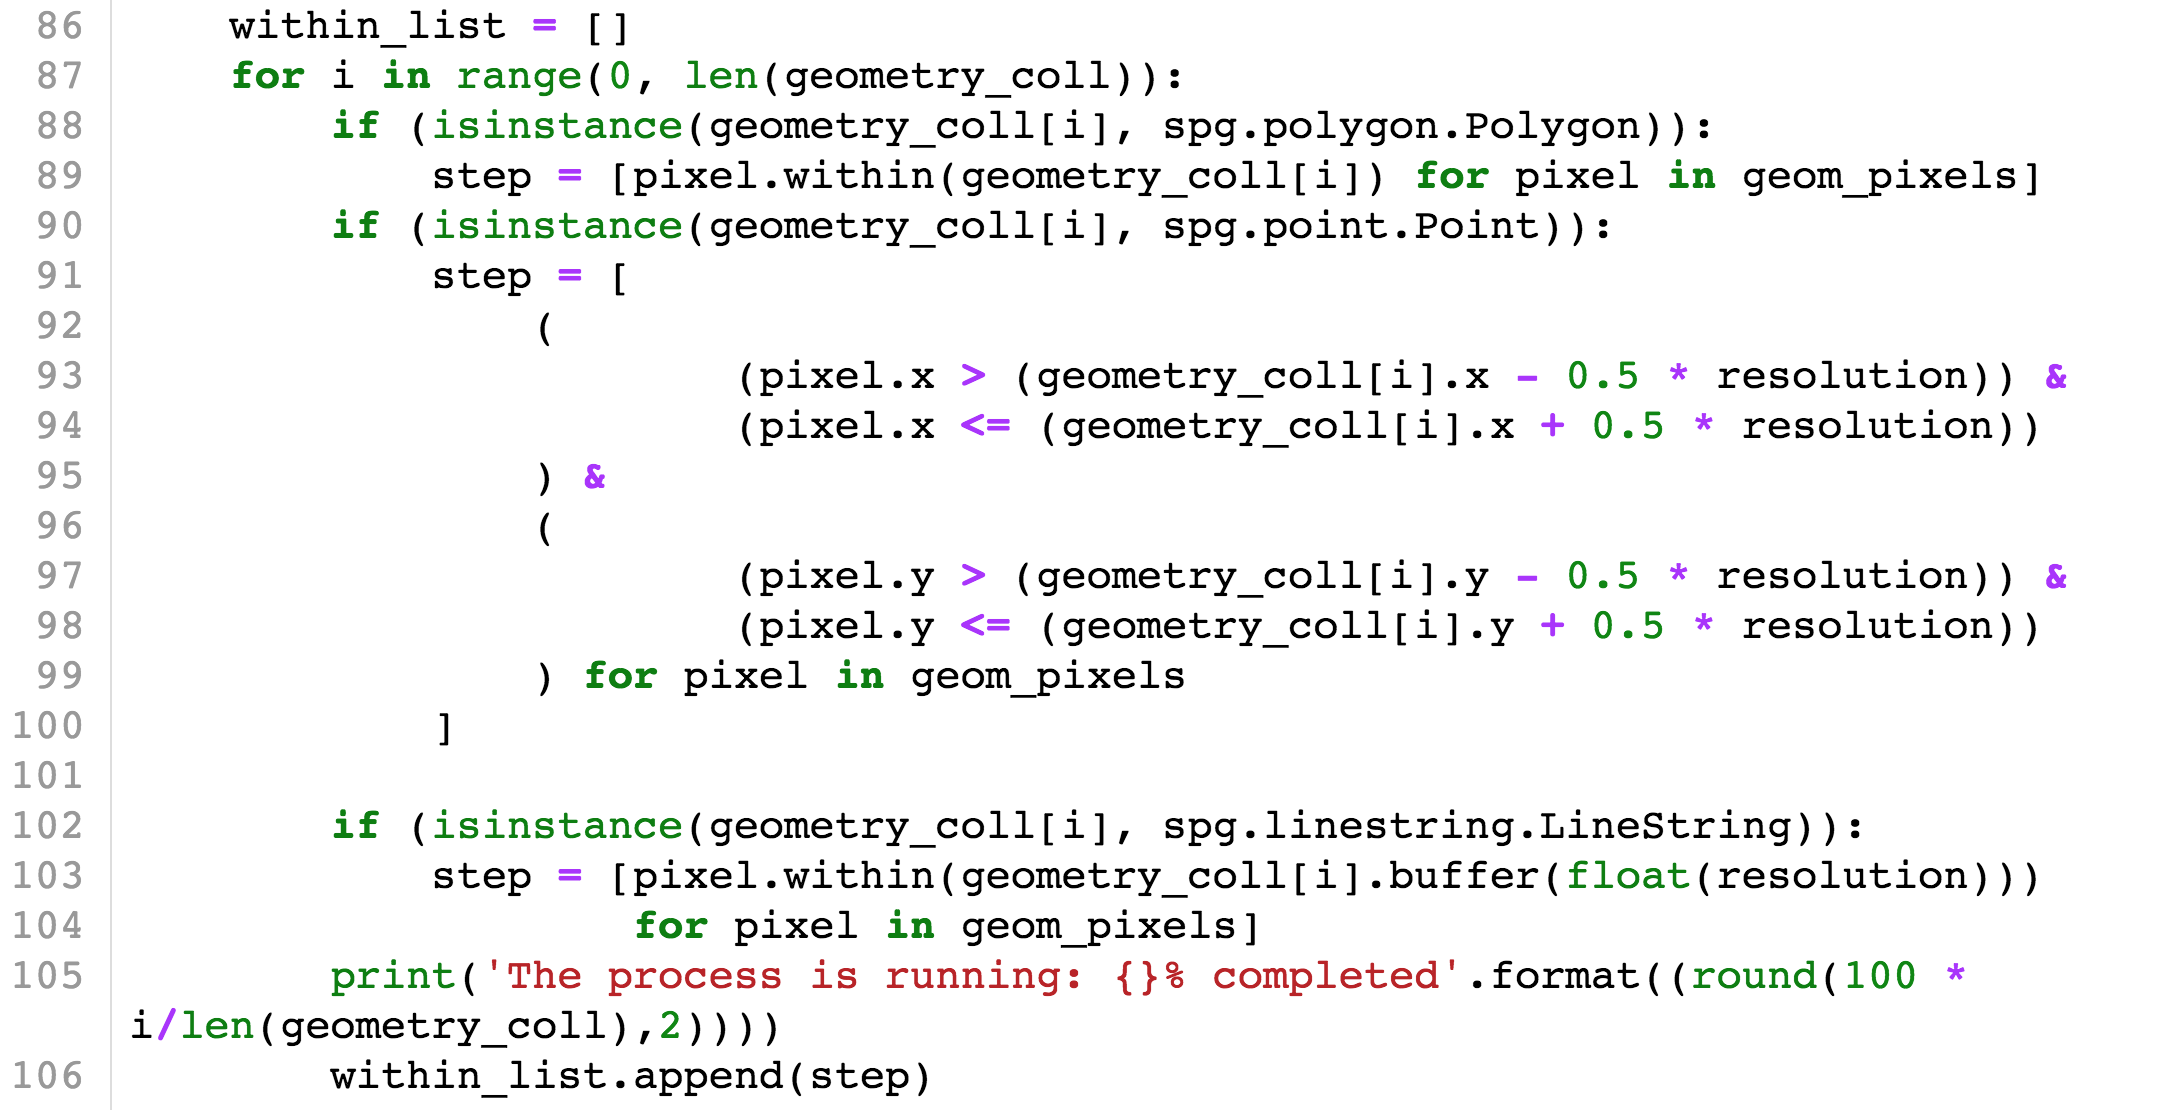
\includegraphics[scale=0.275]{within.png}
\end{frame}


\subsection{Sublist}

\begin{frame}\frametitle{Sublist}
\hspace{0.5cm} 
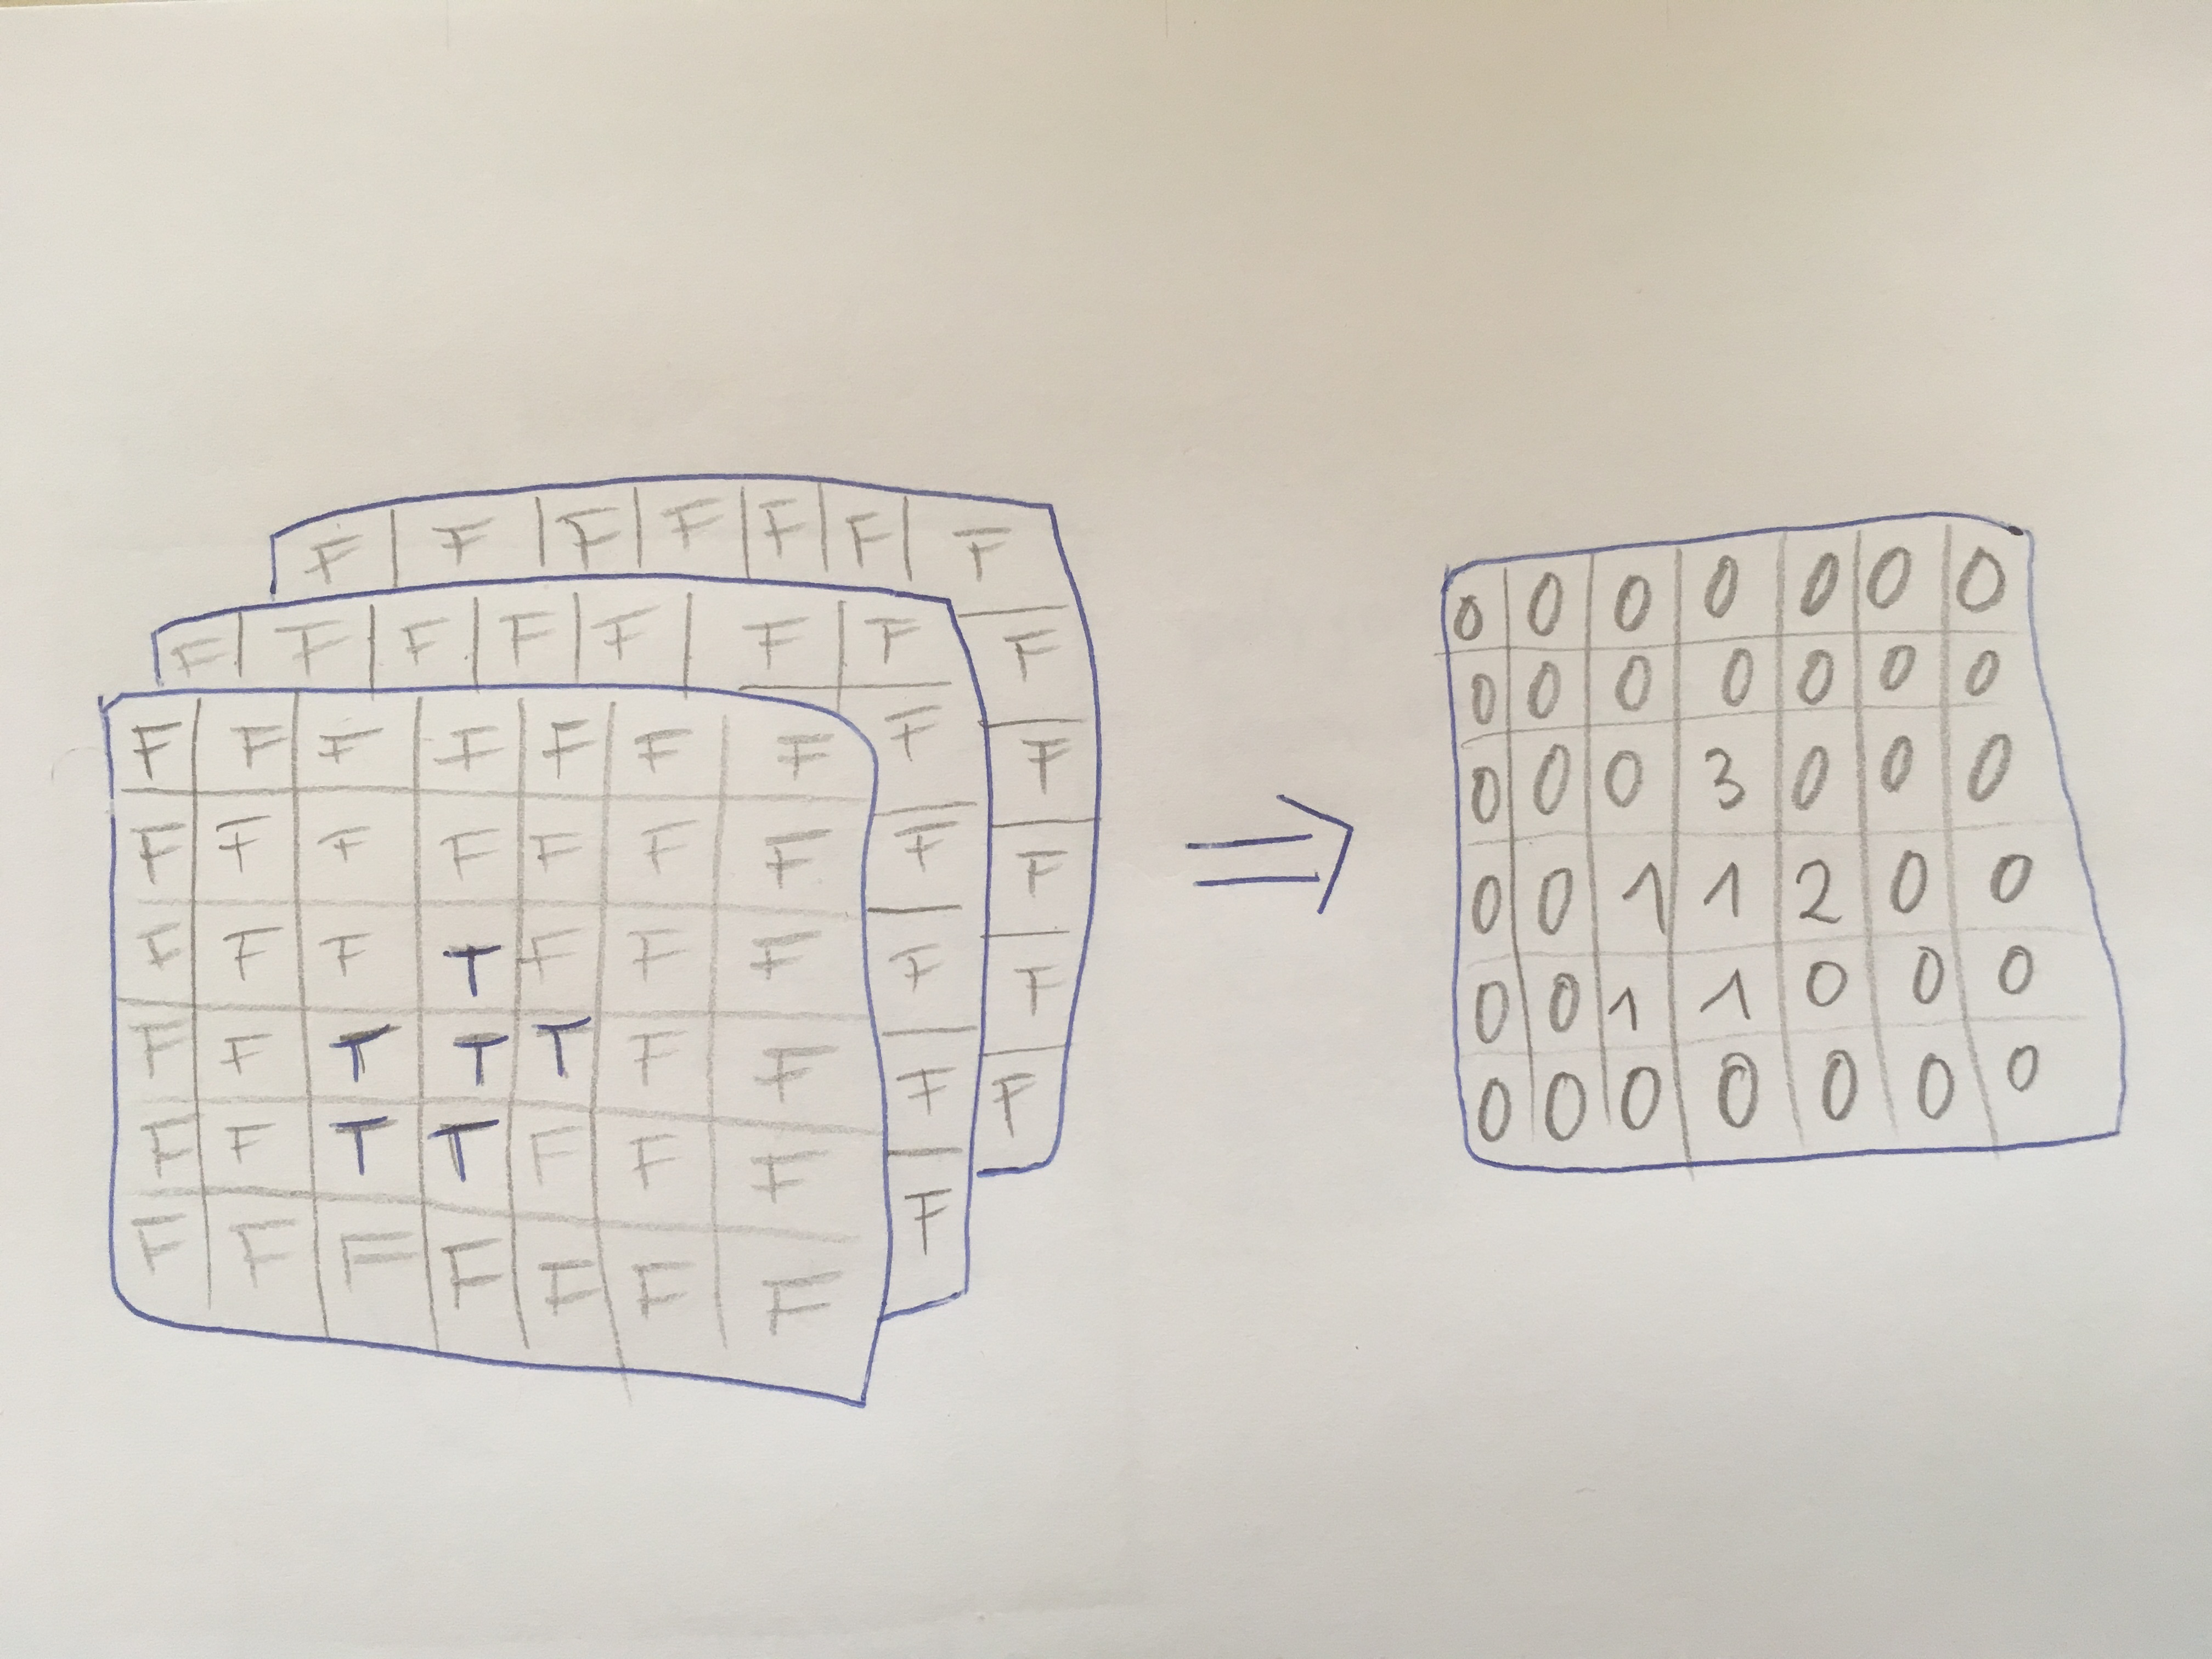
\includegraphics[scale=0.06]{IMG_5504.JPG}
\end{frame}

\subsection{Set radiometric resolution}
\begin{frame}\frametitle{Set radiometric resolution}
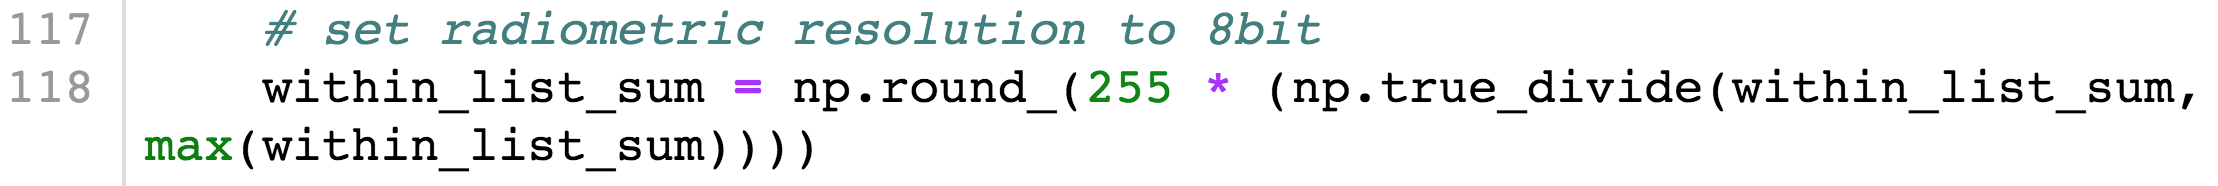
\includegraphics[scale=0.26]{radiometric.png}
\end{frame}

\subsection{Flip array}
\begin{frame}\frametitle{Flip array}
\hspace{0cm} 
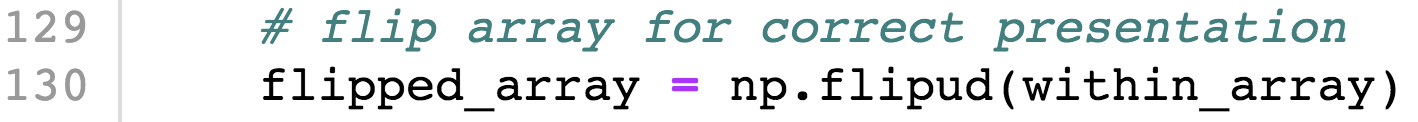
\includegraphics[scale=0.3]{flip.png}
\end{frame}

\subsection{Save as tiff}
\begin{frame}\frametitle{Save as tiff}
%\hspace{0.5cm} 
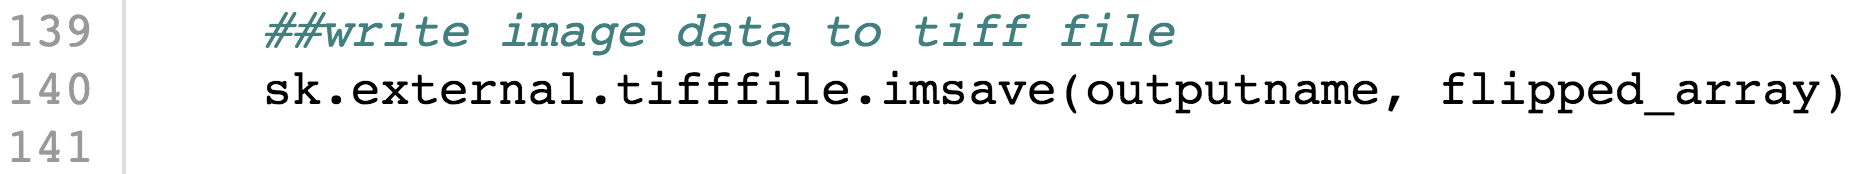
\includegraphics[scale=0.3]{tiffsave.png}
\end{frame}

\section{Issues}
\begin{frame}\frametitle{Issues}
\begin{block}{Solved}
\begin{itemize}
\item Set accurate resolution even if you dont know the range of the coordinates
\item Raster-conversion for shp-types point, line and polygon
\item Git
\end{itemize}
\end{block}
\end{frame}


\begin{frame}\frametitle{Issues}
\begin{block}{unsolved}
\begin{itemize}
\item Save tiff-file with reference-system
\item Define grey-values in tiff-file according to a specific attribute of the shapefile
\item Possibility to choose radiometric resolution of tiff-file 
\end{itemize}
\end{block}
\end{frame}


\end{document}
